\documentclass{article}
\usepackage[margin=1in]{geometry}
\usepackage{setspace, fancyhdr, hyperref, xcolor, tikz, subcaption, float, marginnote}

\usetikzlibrary{positioning, intersections, calc, arrows}
\usepackage[square,numbers]{natbib}
\bibliographystyle{abbrvnat}
\newcommand{\comment}[1]{}
\newcommand{\thetitle}{Symbolic Manipulation and Computation in the Same Graph}
 
\pagestyle{fancy}
\fancyhf{}
\rhead{\thetitle}
\lhead{Darius Barbano}
\rfoot{Page \thepage}
\doublespacing

\author{Darius Barbano}
\title{\thetitle}
\date{}

\begin{document}

\maketitle
\newpage
\tableofcontents
\newpage

\begin{abstract}
    General artificial intelligence refers to machine intelligence than performs a task as successfully as a human does. A fundamental difference between human neural network and current machine neural networks is that only human networks combine symbolic reasoning with computation. \\
    
    In order for neural networks to solve more complex problems, they must be able to manipulate representations of meaningful information. While current networks have been largely successful in a variety of tasks from image classification to sentiment analysis, the internal computations of the networks have only consisted of many basic arithmetic operations. This model is effective in dealing with and taking advantage of relatively transparent patterns in the training data, but in no way does it attempt to develop meaningful representations of the data. To build a model which generates new text based on some previously written text, modern networks would construct (through training) a framework which determines which word has the highest probability of logically making sense given the previous words in the text. These networks have no consideration for the meaning of the words chosen, only their probability of being correct as meaningless objects. For humans, language is anything but a series of meaningless objects called words, rather each word must be understood in terms of it's meaning, connotation, and acceptibility in the context of what is being said. We learn these aspects of the words we use over the course of our lives, and we constantly refer to these memories when choosing which words to use. In the case of human intelligence, each object of understanding (words, concepts, etc) is directly tied to memories and experiences which give them meaning. For neural networks to solve problems with these highly complex objects, they must represent them in a similar fashion. \\
    
\textcolor{red}{- I'm unclear as to whether our focus is to combine Logical symbols and Numerical ones, or to more broadly figure out how to represent complex objects (as stated above)}    
    
\end{abstract}
\newpage


\section{Background}

	Neural networks have been used for decades to solve a wide variety of machine learning tasks without the need for explicit programming of the solutions to be done by humans. Typically the networks only make use of arithmetic computation, meaning that logical operations are not incorportated into the models. This hasn't been done because there is no clear method by which logical information (TRUE/FALSE) should be converted to numerical information, and vice versa. In Computer Science, True and False are generally represented as 1 and 0, respectively, whereas in Mathematics, they are often represented as -1 and 1 \textcolor{red}{Which specific fields of Math and Compsci?}. Our research aims to construct a neural network which effectively combines logical and arithmetic computation, and apply this network to a problem which demostrates it's ability to perform symbolic reasoning.
	
    \begin{enumerate}
        \item What is symbolic computation?
        
        A symbolic computation is a calculation performed with symbolic representations of values and operations. A simple example would be the expression $(x + 1)(x - 1)$ which would evaluate to $x^2 - 1$, rather than to some numerical result.

        \item What is calculation?
        
        A calculation is a process by which one or more inputs is transformed into one or more results. One may calculate that the product of 5 and 4 is 20.
        
        \item What is meant by a computational class? \textcolor{red}{- do you mean complexity class?}
        
        
    \end{enumerate}
    
     Code for each subsection of this document can be found at \href{https://github.com/DariusBxsci/NeuralNetworkResearch/tree/master/NeuralNets}{NeuralNetworkResearch}. 


\section{Methods}

\subsection{Network Construction}

 Figure \ref{fig:sig-neuron} illustrates a neuron that receives three ordered inputs. 

 
 \begin{figure}[!htb]

 \centering
 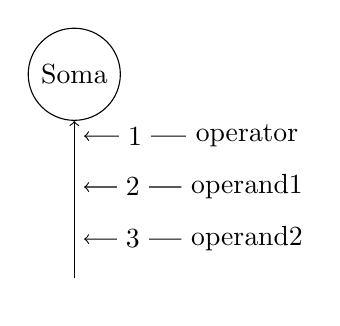
\begin{tikzpicture}

 
    \node[circle, draw=black] (soma) {Soma};
    \node[below= 2cm of soma] (dendrite) {};
    
    \begin{scope}[node distance=1mm and 10mm]
    \node[below right = of soma] (operator) {operator};
    \node[below = of operator] (operand1) {operand1};
    \node[below = of operand1] (operand2) {operand2};
    \end{scope}
    
    
    \draw[->] (dendrite) -> (soma);
    
    
    %nodes along dendrite
    \node (operator'dendrite) at (intersection of operator--soma|-operator and dendrite--soma){};
    
    \node (operand1'dendrite) at (intersection of operand1--soma|-operand1 and dendrite--soma){};
    
    \node (operand2'dendrite) at (intersection of operand2--soma|-operand2 and dendrite--soma){};
    
    
    \draw[->] (operator) -- (operator'dendrite) node[midway, fill=white] {1};
    \draw[->] (operand1) -- (operand1'dendrite) node[midway, fill=white] {2};
    \draw[->] (operand2) -- (operand2'dendrite) node[midway, fill=white] {3};
    
 \end{tikzpicture}
 \caption{Single neuron receiving ordered intputs. \label{fig:sig-neuron}}
\end{figure}


While this model is suitable for biological networks of neurons, a neural network in the computational sense would look more like an abstract syntax tree. In the following diagram, a network of operators and operands form a tree-like structure in which elements at lower levels represent values to manipulate which at higher levels interact with each other through arithmetic operations to produce a result. Any computation which involves a combination of operations on one or more values can be represented in this structure, such as logical or arithmetic operations.


 \begin{figure}[!htb]
 \centering
 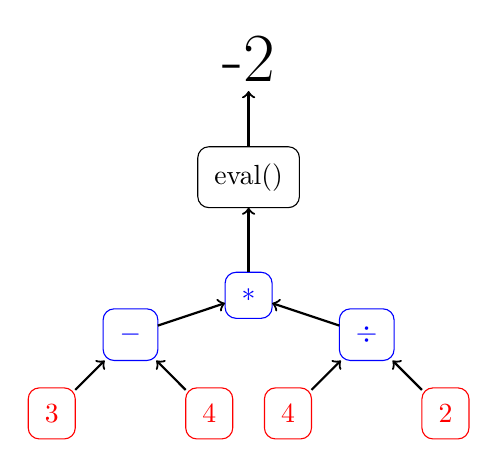
\begin{tikzpicture}

\tikzstyle{bordered} = [shape=rectangle, rounded corners, draw, outer sep=0,inner sep=6,minimum size=15]
\tikzstyle{con} = [thick,->]
\tikzstyle{message} = [shape=rectangle, thick, minimum width=2cm]

	\node [bordered,red] (v1) at (1.5,8) {3};
	\node [bordered,red] (v5) at (3.5,8) {4};
	\node [bordered,red] (v4) at (4.5,8) {4};
	\node [bordered,red] (v3) at (6.5,8) {2};
	
	\node [bordered,blue] (v6) at (5.5,9) {$\div$};
	\node [bordered,blue] (v2) at (2.5,9) {$-$};

	\node [bordered,blue] (v7) at (4,9.5) {$*$};

	\node [bordered,black] (v8) at (4,11) {eval()};

	\node [black] (v9) at (4,12.5) {\Huge -2};

	\draw [con] (v1) edge (v2);
	\draw [con] (v3) edge (v6);
	\draw [con] (v4) edge (v6);
	\draw [con] (v5) edge (v2);

	\draw [con] (v2) edge (v7);
	\draw [con] (v6) edge (v7);

	\draw [con] (v7) edge (v8);

	\draw [con] (v8) edge (v9);

    
 \end{tikzpicture}
 \caption{An Abstract Syntax Tree of arithmetic operations.} 
 \end{figure}

 \begin{figure}[!htb]
 \centering
 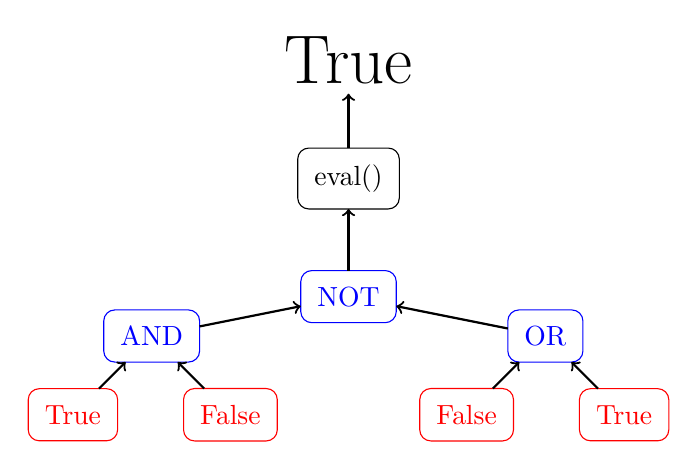
\begin{tikzpicture}
 
 \tikzstyle{bordered} = [shape=rectangle, rounded corners, draw, outer sep=0,inner    sep=6,minimum size=15]
 \tikzstyle{con} = [thick,->]
 \tikzstyle{message} = [shape=rectangle, thick, minimum width=2cm]

	\node [bordered,red] (v1) at (0.5,8) {True};
	\node [bordered,red] (v5) at (2.5,8) {False};
	\node [bordered,red] (v4) at (5.5,8) {False};
	\node [bordered,red] (v3) at (7.5,8) {True};
	
	\node [bordered,blue] (v6) at (6.5,9) {OR};
	\node [bordered,blue] (v2) at (1.5,9) {AND};

	\node [bordered,blue] (v7) at (4,9.5) {NOT};

	\node [bordered,black] (v8) at (4,11) {eval()};

	\node [black] (v9) at (4,12.5) {\Huge True};

	\draw [con] (v1) edge (v2);
	\draw [con] (v3) edge (v6);
	\draw [con] (v4) edge (v6);
	\draw [con] (v5) edge (v2);

	\draw [con] (v2) edge (v7);
	\draw [con] (v6) edge (v7);

	\draw [con] (v7) edge (v8);

	\draw [con] (v8) edge (v9);

    
 \end{tikzpicture}
 \caption{An Abstract Syntax Tree of logical operations.} 
 \end{figure}

\subsection{Using each arithmetic operator with a logical operand} 
{\it Code that corresponds with this section can be found in NeuralNetwork\_5.py}

	Syntax trees such as the ones shown above work perfectly, since each contain exclusively arithmetic or logical computations. In the trees shown below, however, the two computation classes are combined through multiplication and addition. The tree's results depend entirely on how we choose to evaluate $2 * True$ and $2 + True$.
	
	\newpage	
	
 \begin{figure}[!htb]
 \centering
 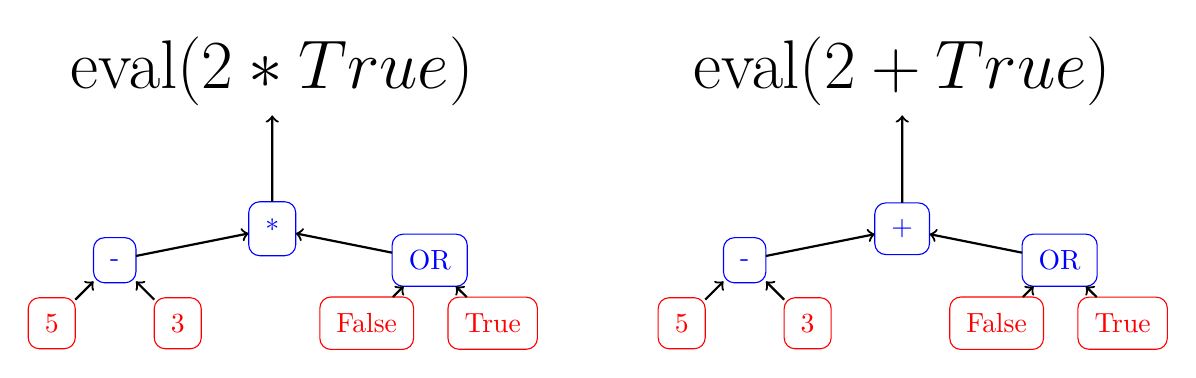
\begin{tikzpicture}[scale=0.8]
 
 \tikzstyle{bordered} = [shape=rectangle, rounded corners, draw, outer sep=0,inner    sep=6,minimum size=15]
 \tikzstyle{con} = [thick,->]
 \tikzstyle{message} = [shape=rectangle, thick, minimum width=2cm]

	\node [bordered,red] (v1) at (0.5,8) {5};
	\node [bordered,red] (v5) at (2.5,8) {3};
	\node [bordered,red] (v4) at (5.5,8) {False};
	\node [bordered,red] (v3) at (7.5,8) {True};
	
	\node [bordered,blue] (v6) at (6.5,9) {OR};
	\node [bordered,blue] (v2) at (1.5,9) {-};

	\node [bordered,blue] (v7) at (4,9.5) {*};


	\node [black] (v9) at (4,12) {\Huge eval($2 * True$)};

	\draw [con] (v1) edge (v2);
	\draw [con] (v3) edge (v6);
	\draw [con] (v4) edge (v6);
	\draw [con] (v5) edge (v2);

	\draw [con] (v2) edge (v7);
	\draw [con] (v6) edge (v7);

	\draw [con] (v7) edge (v9);
	
	
	\node [bordered,red] (vv1) at (10.5,8) {5};
	\node [bordered,red] (vv5) at (12.5,8) {3};
	\node [bordered,red] (vv4) at (15.5,8) {False};
	\node [bordered,red] (vv3) at (17.5,8) {True};
	
	\node [bordered,blue] (vv6) at (16.5,9) {OR};
	\node [bordered,blue] (vv2) at (11.5,9) {-};

	\node [bordered,blue] (vv7) at (14,9.5) {+};

	\node [black] (vv9) at (14,12) {\Huge eval($2 + True$)};

	\draw [con] (vv1) edge (vv2);
	\draw [con] (vv3) edge (vv6);
	\draw [con] (vv4) edge (vv6);
	\draw [con] (vv5) edge (vv2);

	\draw [con] (vv2) edge (vv7);
	\draw [con] (vv6) edge (vv7);
	
	\draw [con] (vv7) edge (vv9);
    
 \end{tikzpicture}
 \caption{Abstract Syntax Trees of logical and arithmetic operations.} 
 \end{figure}

An error would be the result if the two expressions were to be evaluated since $True$ and $False$ are not numerical values so they aren't compatible with numerical operations like $*$ and $+$. Now the question arises, {\it How can logical symbols be converted into numerical values?} In the context of Computer Science and Programming, one may represent $False$ as $0$ and $True$ as $1$. In the case of multiplication, this format would cause $eval()$ to yield $0$ if one of the operands is $False$ and whatever the other operand is if one is $True$. Let us now model a real-world situation in which logical and arithmetic computation are both necessary for a result.

\begin{figure}[H]
 
  \begin{subfigure}{1.0\textwidth}
\centering

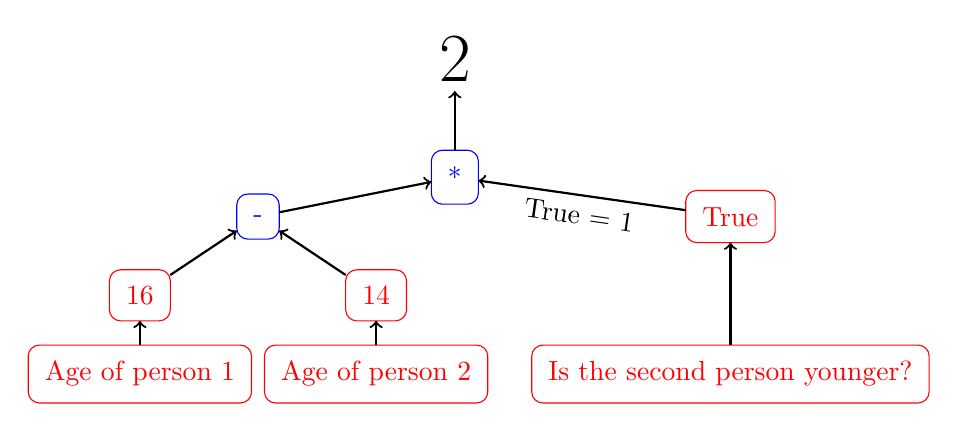
\begin{tikzpicture}

 	\tikzstyle{bordered} = [shape=rectangle, rounded corners, draw, outer sep=0,inner    sep=6,minimum size=15]
 	\tikzstyle{con} = [thick,->]
 	\tikzstyle{message} = [shape=rectangle, thick, minimum width=2cm]

	\node [bordered,red] (vm1) at (0,6.5) {Age of person 1};
	\node [bordered,red] (vm5) at (3,6.5) {Age of person 2};
	\node [bordered,red] (v1) at (0,7.5) {16};
	\node [bordered,red] (v5) at (3,7.5) {14};
	
	\node [bordered,red] (v4) at (7.5,6.5) {Is the second person younger?};
	\node [bordered,red] (v3) at (7.5,8.5) {True};
	
	\node [bordered,blue] (v2) at (1.5,8.5) {-};

	\node [bordered,blue] (v7) at (4,9) {*};


	\node [black] (v9) at (4,10.5) {\Huge 2};

	\draw [con] (vm1) edge (v1);
	\draw [con] (vm5) edge (v5);	

	\draw [con] (v1) edge (v2);
	\draw [con] (v4) edge (v3);
	\draw [con] (v5) edge (v2);

	\draw [con] (v3) edge node[sloped, below] {True = 1}  (v7);

	\draw [con] (v2) edge(v7);

	\draw [con] (v7) edge (v9);
	
\end{tikzpicture}
    
    \caption{First sibling is younger}    
    
  \end{subfigure}
    
  \begin{subfigure}{1.0\textwidth}
  \centering
  
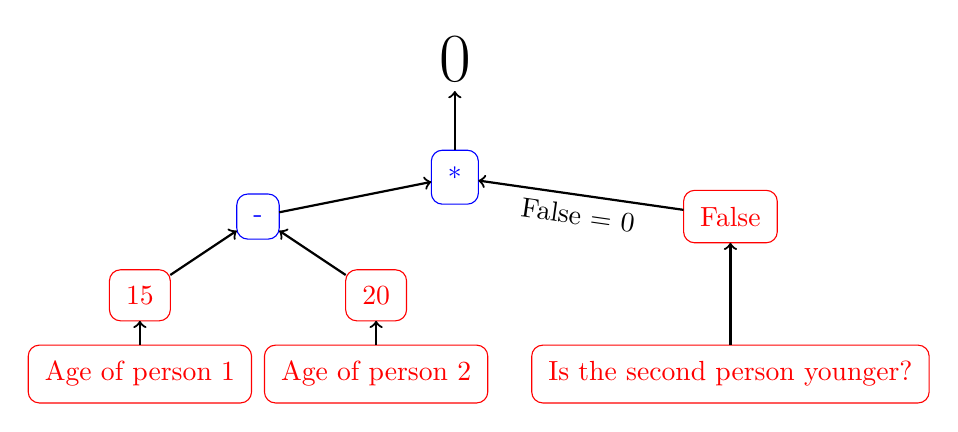
\begin{tikzpicture}

 	\tikzstyle{bordered} = [shape=rectangle, rounded corners, draw, outer sep=0,inner    sep=6,minimum size=15]
 	\tikzstyle{con} = [thick,->]
 	\tikzstyle{message} = [shape=rectangle, thick, minimum width=2cm]

	\node [bordered,red] (vm1) at (0,6.5) {Age of person 1};
	\node [bordered,red] (vm5) at (3,6.5) {Age of person 2};
	\node [bordered,red] (v1) at (0,7.5) {15};
	\node [bordered,red] (v5) at (3,7.5) {20};
	
	\node [bordered,red] (v4) at (7.5,6.5) {Is the second person younger?};
	\node [bordered,red] (v3) at (7.5,8.5) {False};
	
	\node [bordered,blue] (v2) at (1.5,8.5) {-};

	\node [bordered,blue] (v7) at (4,9) {*};


	\node [black] (v9) at (4,10.5) {\Huge 0};

	\draw [con] (vm1) edge (v1);
	\draw [con] (vm5) edge (v5);	

	\draw [con] (v1) edge (v2);
	\draw [con] (v4) edge (v3);
	\draw [con] (v5) edge (v2);

	\draw [con] (v3) edge node[sloped, below] {False = 0}  (v7);

	\draw [con] (v2) edge(v7);

	\draw [con] (v7) edge (v9);
	
\end{tikzpicture}  
  
    \caption{Second sibling is younger}
    
  \end{subfigure}
  
 \caption{A syntax tree which models how many years one person is older than another, using a combination of Arithmetic and Logical computation.} 
 \end{figure}
 
 
 In the above trees, logical and numerical information are effectively combined to produce an output. If only numerical information were used (i.e. the ages of the two people), only the difference of the two numbers would be calculated, yielding $-5$ in the second case. However, a person cannot be a negative number of years older than another, so $0$ would be a more appropriate result. The above trees solve this problem by requiring the user to give a boolean value representing whether or not the second person is younger than the first, then the $True/False$ value is converted into a number according to previously defined policy and multiplied with the difference of the two ages. \\
 
 We have just successfully formulated a method by which logical symbols and numbers can be combined through the multiplication operator, but how would the two be combined through the subtraction, division, and addition operators? \\
 
 The process of multiplication can be broken down into a series of repeated additions. For example, $4 * 3$ is the same as $4 + 4 + 4$. Therefor, the expression $4 * True$ can be broken down into $True + True + True + True$. Let us add $True$ to this expression and get $True + True + True + True + True$, and simplify it to just $5 * True$ (by the distributive property of multiplication), which by our multiplication rule would evaluate to $5$. By this logic, adding $True$ to a value is equivalent to adding $1$, and adding $False$ is equivalent to adding $0$. We can extend this to subtraction, so that subtracting $True$ subtracts $1$ and $False$ subtracts $0$ \\

 The division and multiplication operators are inverse operations. In other words, if a number is divided by number, $x$, multiplying the result by $x$ would yield the original number. Naturally, this relationship should remain when using logical operands. However, this poses a major problem since if a value is multiplied by $False$, the output will be $0$, and there is no number that $False$ can be converted into such that dividing $0$ by it will yield the initial value (if the initial value is not $0$).
\textcolor{red}{- How can/should this problem be reconciled?} \\

\subsection{An alternative solution}

	In the previous subsection, we attempted to solve the problem of combining logical and numerical symols by converting $True$ into $1$ and $False$ into $2$. In doing this, we noticed that the multiplication operator could be used with a logical symbol to either propogate or to destroy a numerical signal. On the other hand, we were not able to put the addition, subtraction, and division operators to meaningful use, as we were with multiplication. From these results, it should be clear that an alternative solution is necessary. To discover this solution, we will examine a few situations where the two brands of computation are necessary, and formulate how the two can be combined into one family of computations. 
	
(a tree which models a situation where logical and numerical information need to be combined via some operator) \textcolor{red}{- What sort of situation REQUIRES this? (TemperatureTree is a possibility)}

	It is unclear how the two should be combined such that the meaning behind each value is retained. In the above situation... (describe how one would combine the two in the above situation to yield the correct output). \\ \\
	
	\textcolor{red}{Ideas for solving the problem of combining the two forms of information:}
	
\begin{enumerate}

\item The simplest solution would be to simply convert all information into one type, rather than having them be separate. The issue with this that the converted information may lose it's representational meaning.

\item Another solution would be to store all information as a tuple with a numerical element and a logical element. Numerical operations would exclusively act on numbers and logical operations on logical symbols.

\item Some new data structure could be made which exists as a postion in space, where one dimension describes logical state and the other describes numerical state. Similar to points on a cartesian plane, except the 'x' axis would be True/False, and the 'y' axis would be a numerical value. Operations could be performed on this object as transformations in the same way they could be done to points on an xy plane. This solution could be advantageous in the long run since any new data type can be added to the data structure by adding a new dimension for it and tranforming points in operations in the same way.

\end{enumerate}


\section{Results}

\section{Conclusions}

\bibliography{references}

\end{document}